\begin{tikzpicture}[x=1cm,y=1cm,font=\normalsize,
 geometry edge/.style={solid,line width=.6pt},
 geometry mark/.style={solid,line width=.6pt},
 geometry label/.style={font=\normalsize,inner sep=2pt}]
\coordinate (R1) at (0,0);
\coordinate (R2) at (2.25,0);
\coordinate (R3) at (2.25,4.5);
\coordinate (R4) at (0,4.5);
\coordinate (Q1) at (0,1.5);
\coordinate (Q2) at (2.25,1.5);
\coordinate (Q3) at (0,3);
\coordinate (Q4) at (2.25,3);
\draw[geometry edge] (R1)--(R2)--(R3)--(R4)--cycle;
\draw[geometry edge] (Q1)--(Q2);
\draw[geometry edge] (Q3)--(Q4);
\draw[geometry mark,decorate,decoration={brace,amplitude=6pt,mirror}] (2.55,0)--(2.55,4.5);
\draw[geometry mark,decorate,decoration={brace,amplitude=6pt,mirror}] (0,-0.3)--(2.25,-0.3);
\node[font=\normalsize,inner sep=2pt] at (3.2,2.25) {$x$};
\node[font=\normalsize,inner sep=2pt] at (1.125,-1.05) {$\dfrac{6-2x}{4}$};
\end{tikzpicture}
